\documentclass[11pt]{article}
\usepackage{amsmath}
\usepackage{amssymb}
\usepackage{graphicx}
\usepackage{epstopdf}
\usepackage{inputenc}
\usepackage{float}
\usepackage{geometry}
\graphicspath{ {../results/plots} }
\usepackage{csvsimple}
\usepackage{hyperref}
\usepackage{listings}
\usepackage{cleveref}
\usepackage{lscape}

\newcommand{\betaEst}{0.184}
\newcommand{\rhoEst}{364}
\newcommand{\repEst}{6.04}
\newcommand{\RN}[1]{%
  \textup{\uppercase\expandafter{\romannumeral#1}}%
}

\title{SARS-CoV-2 Outbreak Reduction: Executive Summary}

\author{
        Forrest Koch \\
        forrest.koch@unsw.edu.au \\
        University of New South Wales \\
}
\date{\today}

\begin{document}
\maketitle

\section{Executive Summary}
The global pandemic caused by SARS-CoV-2 has so far resulted in over 100 million infectious and 2 million deaths worldwide 
\cite{noauthor_who_nodate}.  It has had an enormous impact on the global economy. There was estimated 8.8\% decrease in 
global working hours throughout 2020 and losses are expected to continue into 2021 \cite{noauthor_ilo_2021}.  Given
the scale and magnitude of this pandemic, it is essential that government policy makers are well informed as to
what the most effective management strategies are for combating this infectious disease.  Furthermore, it is important
to evaluate previous policy decisions in order to determine their efficacy and appropriateness for future use.

In March of 2020, California, the most populous state in the U.S, entered its first wave of the pandemic.  This
was followed by a stream of policies aimed to reduce transmission of the disease (see Table \ref{wiki_table} for a summary).
It would appear that these measures were successful as the number of new cases gradually started to decrease after July.

In this work, we used data provided by the California Department of Public Health (CDPH) to model the transmission of 
SARS-CoV-2 between April 7, 2020 and October 4, 2020. We found that there was a 23\% decrease in the rate of transmission 
over this time period. This corresponds to a decrease in the effective reproduction number from 1.289 to 0.914 and indicates
the policies were successful in reducing the spread of SARS-CoV-2.

Furthermore, we calculated
$R_0$, the basic number of reproduciton,  at 1.29 which would suggest that an effective vaccination rate of around 23\% would be sufficient to limit the spread of
SARS-CoV-2 in the Californian population; however, these figures do not agree with the existing literature.  This underestimation is likely due to an
artificially low rate of transmission at the beginning of the period being studied.

Due to the limited time for this work, further research and funding is recommended in order to provide 
more conclusive answers.  This work has several limitations
that must be addressed before it is used to inform policy, however, the information presented here aims to pave the way for
this future work.  This includes, but is not limited to stratifying the population by demographic and location in order to
determine optimal vaccination strategies. 

    \begin{table}[H]
        \begin{tabular}{p{.25\linewidth}|p{.75\linewidth}}
            Date 	& Action Taken \\
            \hline \\
            March 4, 2020 & 	State of emergency declared. \\
            March 12, 2020 & 	Mass gatherings (over 250 people) and social gatherings (over 10 people) banned. \\
            March 19, 2020 & 	State-wide stay-at-home order issued. \\
            March 24, 2020 & 	Intakes in prisons and juvenile correction centers postponed. \\
            April 1, 2020 & 	Closure of all public and private schools (including institutions of higher education) ordered for the remainder of the 2019–2020 academic year. \\
            April 9, 2020 & 	State offered to pay hotel room costs for hospital and other essential workers afraid of returning home and infecting family members. \\
            April 24, 2020 & 	Program to deliver free meals to elderly residents announced. \\
            April 29, 2020 & 	Expansion of the state's Farm to Family program (which helps connect farmers to food banks) announced. \\
            May 6, 2020 & 	Worker's compensation extended for all workers who contracted COVID-19 during the state's stay-at-home order. \\
            May 6, 2020 & 	Property tax penalties waived for residents and small businesses that have been negatively affected by the pandemic. \\
            May 7, 2020 & 	State entered Stage 2 of its 4-stage reopening roadmap. \\
            May 8, 2020 & 	Executive order signed that would send every registered voter a mail-in ballot for the general election. \\
            May 18, 2020 & 	Businesses that are part of Stage 3 allowed to reopen. \\
            May 26, 2020 & 	Hair service businesses allowed to reopen (with restrictions). \\
            June 18, 2020 & 	Universal masking guidance issued by Department of Public Health. \\
            June 28, 2020 & 	Bars ordered to close in several counties. \\
            July 1, 2020 & 	Most indoor businesses, including restaurants, wineries, and movie theaters ordered to close in several counties. \\
            July 13, 2020 & 	Closure of gyms, indoor dining, bars, movie theaters, and museums re-imposed. \\
            August 28, 2020 & 	Unveiled a new set of guidelines for lifting restrictions, titled a "Blueprint for a Safer Economy". \\
            August 31, 2020 &	BSE county-level restrictions take effect. See below for initial classifications. More than 80\% of population is under "Widespread" restrictions. \\
            September 29, 2020 & Majority of population now under "Substantial" or lower BSE restrictions
        \end{tabular}
        \caption{Table of California Government response taken from wikipedia (\url{https://en.wikipedia.org/wiki/COVID-19\_pandemic\_in\_California\#Government\_response})}
        \label{wiki_table}
    \end{table}
\section{Project Scope}
\subsection{Overall Description}
The aim of this project is to assess the effectiveness of the policies introduced during the 07/04/20-04/10/20 outbreak of
SARS-CoV-2 in California, and to provide recommendations for policy makers to how subsequent outbreaks should be handled.
Daily reports of Covid-19 cases over this time period will be used to construct a transmission model specific to the 
Californian population.  The information gained from the model can then be used to assess whether policies were effective
in reducing transmission as well as estimate what rate of vaccination would be been sufficient to prevent the outbreak.

\subsection{Outcomes}
This project will provide an estimate of the change in transmission rate over the time course of the outbreak. This will
allow us to determine how effective the government-introduced policies in Table \ref{wiki_table} were.

Furthermore,
the basic reproduction number, $R_0$, will be estimated for the Californian population, allowing for an estimation of the
vaccination rate that would have been sufficient to prevent the outbreak.

\subsection{Justification}
As previously discussed, SARS-CoV-2 has had an unprecedented impact on the global economy, and California has not managed to
escape this \cite{noauthor_economics_nodate}. As such, it is imperative that policy makers remain well-informed as to what
the best infection disease management solutions are.  This includes evaluating the effectiveness of past decisions in order
to determine whether they should be repeated.

\subsection{Limitations and Assumptions}
The time and workforce available for this project are severely limited. As such, the original scope of this project has had 
to be reduced to allow for a timely completion. Originally, it was planned to include ethnicity, age, and other demographic
information in the model to provide more detailed information.  Additionally, spatial information and variation in population
behavior are ignored leading to the assumption that the entire population of California as homogenous, which is clearly not the case.

Furthermore, due to the large number of policies introduced during the 
time period of interest, it will not be possible to determine to what extent each of them contributed to reduced 
transmission, and more targeted, agent-based, models would need to be developed in order to address this question.

Daily reports of Covid-19 cases will be used as an estimate of disease incidence, however, these are an underestimate of the
true incidence. Furthermore, this data doesn't technically represent incidence as it captures individuals at different stages
of the infection.

Also, due to the short time period being considered, demography (births and deaths), will be ignored, as will deaths due to
Covid-19.

\section{Approach}
\subsection{Model Description}
The approach to this project is described in detail in the Technical Appendix (Section \ref{appendix}). 
We began by adapting the compartmental transmission model proposed by 
Radulescu et. al. (2020)\cite{radulescu_management_2020}.  In this model, individuals are considered has having 1 of 6 
possible state.  In the first state, $S$, individuals are susceptible to disease.  In the latent state, $L$, individuals
have been exposed to SAR-CoV-2, but are minimally infectious. This state is assumed to last around 4 days.  
From here, they can go on to develop an asymptomatic infection or a symptomatic infection. The asymptomatic infection 
(state $A$) lasts around 12 days during which time they are still minimally infectious.  The symptomatic infection begins with
a pre-symptomatic stage, $P$, for around two days during which time the individual is hyper-infectious. This is followed by 
period of moderate infectiousness for around 10 days.  All infected individuals eventually enter a recovered state, $R$.

\subsubsection{Our Improvements}
We improved on this model making the duration of infection more 
realistic. This was done by allowing infection times to follow a Gamma distribution instead of an Exponential distribution,
as has been observed in medical research \cite{brauer_mathematical_2019}.  A flow diagram for the transmission model is 
available in Figure \ref{flow_diagram}.

Finally, another modification to the model allowed us to vary the rate of transmission over time. This is what allows
us to estimate the change in the rate of transmission between the beginning and end of the outbreak.

\subsubsection{Estimation of Outcomes}
The majority of the parameters used in this model were taken from the work of Radulescu et. al (2020); however, the time-varying 
rate of transmission, $\beta_{eff}(t)$, needed to be calibrated for the Californian population.  This was done using 
daily reports of Covid-19 in California alongside Approximate Bayesian Computational methods.  These methods are very
computationally expensive, but allow for the calculation of credible intervals for very complicated models.

With an estimation of $\beta_{eff}(t)$, we can directly estimate the change in transmission rates, effective (and basic) 
reproduction numbers, as well as the necessary rates of vaccination which would have prevented the outbreak.

\section{Results}

    Table \ref{outcomes_table} gives estimates and descriptions for each outcome of interest. In particular, we
    estimate that the policies introduced by the Californian government reduced transmission by around 29\%,
    lowering the effective reproduction number to $0.9$.  Noteably, this is less than 1 which is necessary for
    stopping viral spread.

    Furthermore, we estimated $R_0$ at 1.29 for this population, indicating that a vaccination rate of 23\% may
    have been sufficient to prevent the outbreak.  However, it should be noted that the movement of individuals was
    likely already decreased at the beginning of the period of study, so this value may not hold for a "normal" population.

    \begin{table}[H]
        \begin{tabular}{ c l l l}
            Outcome of Interest     & Description                                   & Value \\
            \hline \\
            $\beta_{start}$         & The initial rate of transmission              & $0.11547 \pm 3.2\times10^{-5}$ \\
            $\beta_{end}$           & The initial rate of transmission              & $0.08164 \pm 5.3\times10^{-5}$ \\
            $\beta_{fraction}$      & Percentage decrease in transmission           & $29.294 \pm .063\%$ \\
            $R_0$                   & Basic reproduction number                     & $1.2932 \pm 3.6\times10^{-4}$ \\
            $R_{eff-end}$           & Effective reproduction number after outbreak  & $0.9144 \pm 5.9\times10^{-4}$ \\
            $1-\frac{1}{R_0}$       & Minimum rate of necessary vaccination         & $22.676 \pm .021\% $
        \end{tabular}
        \caption{Table of outcomes of interest}
        \label{outcomes_table}
    \end{table}

    Figure \ref{model_fit} shows predicted incidence versus observed cases. We observe a very tight credible interval which
    is unusual for this sort of model and may require further inspection.  The model appears to provide a relatively good fit,
    but underestimates the peak number of cases.

    Figure \ref{beta_over_time} shows the estimated change in transmission rates over time. The change appears to occurr
    over a period of around 30-40 days.

    \begin{figure}
        \centering
        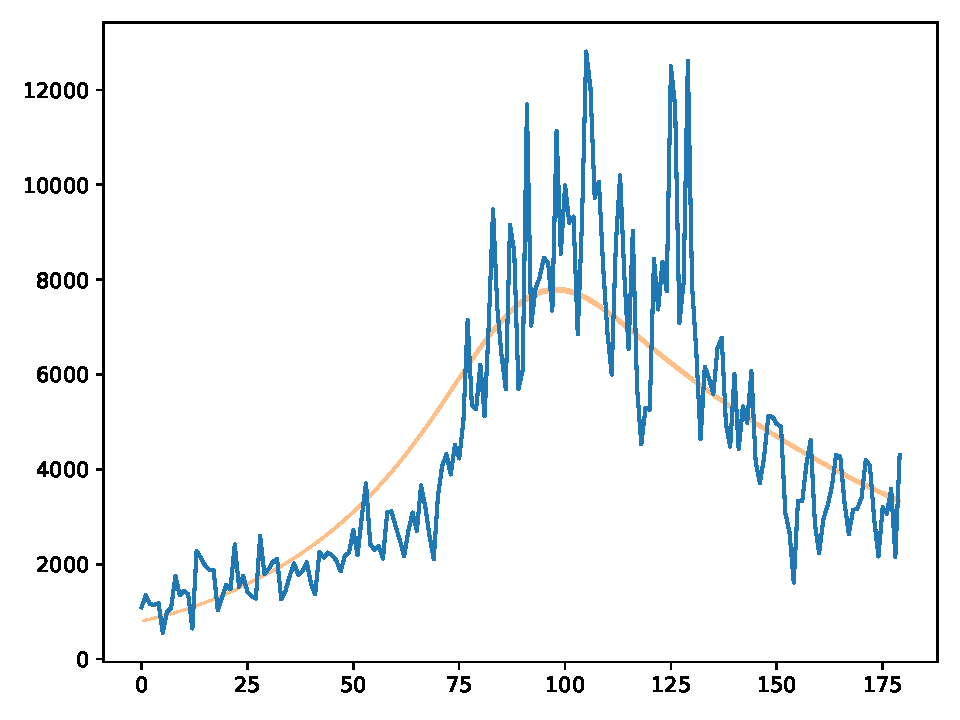
\includegraphics[scale=0.75]{model_fit}
        \caption{Plot of daily reports of Covid-19 cases in California over 180 days starting from 07/04/20-04/10/20 (blue) 
        and the incidence predicted by the model fit with 95\% HDI (orange).}
        \label{model_fit}
    \end{figure}

    \begin{figure}
        \centering
        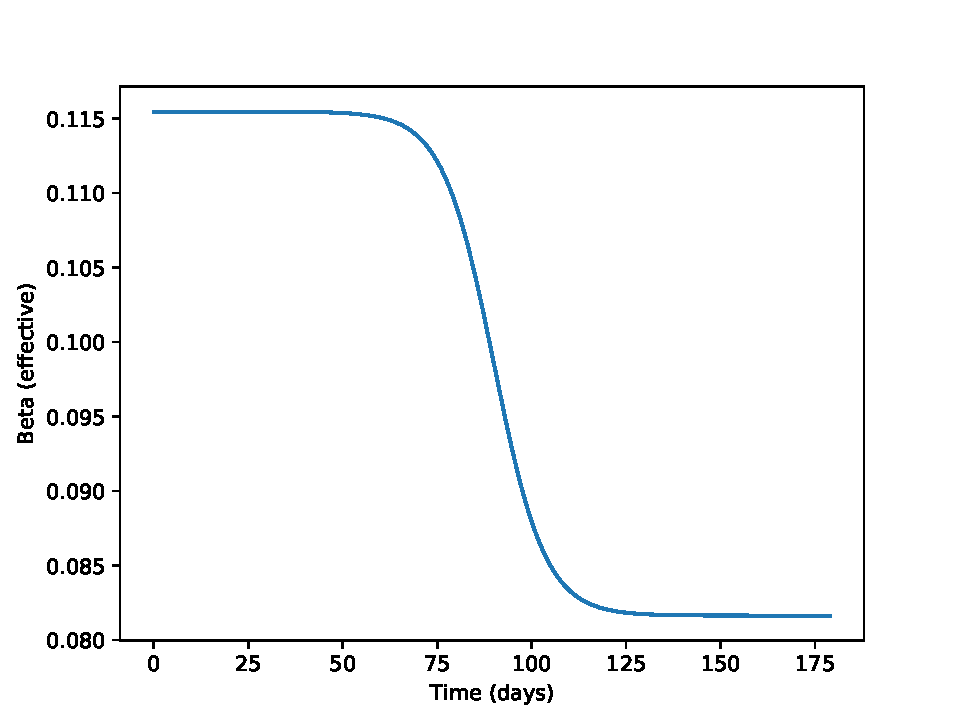
\includegraphics[scale=0.75]{beta_over_time}
        \caption{Plot of the estimated change it $\beta_{eff}$ over the period studied.}
        \label{beta_over_time}
    \end{figure}

\section{Limitations}
    This work possess several limitations that should be taken into consideration when reviewing the results.
    Most importantly, our estimate of $R_0$ (1.29) varied drastically from what is commonly reported in literature (2.5) 
    \cite{davies_age-dependent_2020}. Using an $R_0$ of 2.5 suggested that 60\% of the population should be effectively 
    vaccinated to reduce transmission. Given the dangers associated with outbreak, it is suggested that policy makers
    use more conservative estimates when considering vaccination strategies.

    Furthermore, the model employed by this project produced suspiciously small credible intervals.  This
    should be investigated further to rule out a potentially faulty model.  Additionally, no sensitivity analysis has
    been performed, and so the impact of certain model assumptions is still unknown.

\section{Recommendations}
    Our model suggests that the rate of transmission was decreased by 29\% throughout the course of the outbreak.
    This was sufficient to stop the spread of SARS-CoV-2. As such, policy makers are encouraged to consider implementing 
    the policies imposed during the course of the first outbreak between April and October of 2020 in California in order to
    prevent future outbreaks. In particular, we estimated a sharp decline in transmission around July of 2020 (see Figure 
    \ref{beta_over_time}), so it may be worth investigating the policies introduced around this time further (see Table 
    \ref{wiki_table}).

    Due to the large limitations of this work, we do not advise that any decisions are made based on this project alone.
    More work is necessary to solidify our conclusions.

\section{Future Work}
    Future work should explore the effects spatial, demographic, and behavioral heterogeneities on rates of transmission.
    This will allow us to determine optimal strategies for managing potential outbreaks by suggesting target groups for
    intervention. This would mean that management strategies can be implemented as cost and time efficiently as possible.

    Furthermore, stochastic models should be used in the work in order to better quantify the probability of different 
    outcomes.  The models presented in this work are purely deterministic. This was not an issue in this project, as the
    population is assumed to be large and homogeneous; however, the proposed subdivisions in the population would likely
    make such models prone to random variation.

\section{Technical Appendix}\label{appendix}

\subsection{Methods}
\subsubsection{Data}
    Data for daily reports of Covid-19 cases were acquired from the Californian Department of Public Health (CDPH)
    \cite{noauthor_covid-19_nodate}, and a period of 180 days (07/04/20-04/10/20) was extracted to study the first wave
    of infections. This time frame was selected as it is the period of the first outbreak in California, with the peak
    occuring halfway, or 90 days, in.  These reports of new cases were taken as an estimate of the disease incidence.

\subsubsection{Model Description}
    \begin{figure}
        \centering
        \includegraphics[scale=0.75]{flow_diagram}
        \caption{Flow diagram of the SLAPIR compartmental model. Multiple compartments are leveraged to enforce a gamma 
        distribution on total time spent in the compartment.  Infected individuals go through a latent period (L1-4) followed by
        either an asymptomatic period (A1-12, probability = 20\%) a pre-symptomatic/symptomatic period (P1-2/I1-10, probability = 80\%).}
        \label{flow_diagram}
    \end{figure}
    We developed a transmission model based on the SLAPIR model proposed by Radulescu et. al. (2020)\cite{radulescu_management_2020}. This model contains 6 primary compartments: $S$, for susceptible individuals; $L$, for latent infections; $A$, for 
    asymptomatic infections; $P$, for pre-symptomatic infections; $I$, for symptomatic infections; and $R$ for recovered 
    individuals. 

    It is known that infection periods tend to follow a gamma distribution instead of the exponential distribution
    predicted by a compartmental model \cite{brauer_mathematical_2019}. For this reason, we included multiple sub-compartments
    for each of the infection states ($L,A,P,I$) each with a rate of 1. The number of sub-compartments for each infection
    state was determined from prior literature (see Table \ref{parameter_table}).

    To account for changes in human behavior over the course of the outbreak, we allow the effective rate of transmission 
    $\beta_{eff}$ to vary over time according to the logistic function
    $$\beta_{eff}(t) = \beta_{end} + \frac{\beta_{start}-\beta_{end}}{1+e^{-k(m-t)}}$$
    where $\beta_{start}$ is the initial rate of transmission, $\beta_{end}$ is the final rate of transmission, $m$ is
    the inflection point, and $k$ is a steepness parameter determining how quickly this transition occurs.

    \begin{table}
        \begin{tabular}{ c l l l}
            Parameter & Description & Value \\
            \hline \\
            $\beta_{eff}(t)$       & The effective transmission rate at time $t$            & estimated from data \\ 
            $Q_I$                   & Transmission scaling factor for state $I$                     & 1 \\
            $Q_A$                   & Transmission scaling factor for states $A$ and $L$            & 0.2 \\    
            $Q_P$                   & Transmission scaling factor for state $P$                     & 1.2 \\
            $N_L$                   & Duration of latent period (number of compartments)            & 4 \\
            $N_A$                   & Duration of asymptomatic period (number of compartments)      & 12 \\
            $N_P$                   & Duration of pre-symptomatic period (number of compartments)   & 2 \\
            $N_I$                   & Duration of symptomatic period (number of compartments)       & 10 \\
            $N$                     & Population size                                               & $39\times10^6$ \\
            $\alpha$                & Asymptomatic incidence                                        & 0.2 
        \end{tabular}
        \caption{Table of parameters used in the model. Unless otherwise specified, these parameters were take from Table 1
        from Radulescu et. al. (2020)\cite{radulescu_management_2020}}
        \label{parameter_table}
    \end{table}

\subsubsection{Model Equations}
    The transmission model was implemented as the following system of differential equations:
    \begin{flalign}
        \frac{dS}{dt} &= -\beta_{eff}(t)\Big(Q_A\sum_{i=1}^{N_L}L_i + Q_A\sum_{i=1}^{N_A}A_i + Q_I\sum_{i=1}^{N_I}I_i + Q_p\sum_{i=1}^{N_P}P_i\Big) \\
        \frac{dL_1}{dt} &= \beta_{eff}(t)\Big(Q_A\sum_{i=1}^{N_L}L_i + Q_A\sum_{i=1}^{N_A}A_i + Q_I\sum_{i=1}^{N_I}I_i + Q_P\sum_{i=1}^{N_P}P_i\Big) - L_1 \\
        \frac{dL_i}{dt} &= L_{i-1} - L_i \\
        \frac{dA_1}{dt} &= \alpha L_4 - A_1 \\
        \frac{dA_i}{dt} &= A_{i-1} - A_i \\
        \frac{dP_1}{dt} &= (1-\alpha) L_4 - P_1 \\
        \frac{dP_2}{dt} &= P_{1} - P_2 \\
        \frac{dI_1}{dt} &= P_{2} - I_1 \\
        \frac{dI_i}{dt} &= I_{i-1} - I_i \\
        \frac{dR}{dt}   &= I_{10} + A_{12} 
    \end{flalign}

\subsection{Approximate Bayesian Computation of $\beta_{eff}(t)$}
    The model described above was implemented in STAN \cite{carpenter2017stan} using the following priors:
    \begin{flalign}
        \beta_{start}   &\sim Cauchy(0,0.25) \\
        \beta_{prop}    &\sim Beta(2,2) \\
        \beta_{end}     &= \beta_{start}\times\beta_{prop} \\
        k               &\sim Beta(2,8)
    \end{flalign}
    The prior for $\beta_{start}$ was chosen as the Cauchy is a weakly informative prior, providing minimal bias to the fit.
    $\beta_{prop}$ was sampled between 0 and 1 to enforce a reduction in transmission (as is apparent in the data), and $k$ 
    was chosen to prefer more gradual transitions because an abrupt change is unrealistic. Furthermore, a Poisson likelihood
    was used for the incidence of the model, where incidence is defined as the number of individuals entering the $I_1$ 
    compartment. Note that this represents disease incidence, not infection incidence.

    This model was then estimated using STAN's default Hamiltonian Markov Chain (HMC) algorithm \cite{standev2018stancore}. 18 chains were run for 21,000
    iterations with a burn in period of 1,000. Chains were checked for autocorrelation (see Figure \ref{model_autocorrelation})
    and convergence (see Figure \ref{model_rank} and R\_hat in Section \ref{stansummary}).

\subsection{Bayesian Model Output Summary}
\lstinputlisting[basicstyle=\tiny]{../results/stansummary-clean.txt}\label{stansummary}

\subsection{Calculation of $R_0$}
We used the next-generation matrix method of computing $R_0$ \cite{brauer_mathematical_2019}.
Due to the number of compartments, the closed form for this model is complicated to write down, so the following
code was used for calculations. With $\beta=0.1154$, we get $R_0\approx1.29$.

\lstinputlisting[language=python,basicstyle=\tiny]{../src/basic_reproduction_number.py}


\subsection{Supplemental Figures}
    \begin{figure}
        \centering
        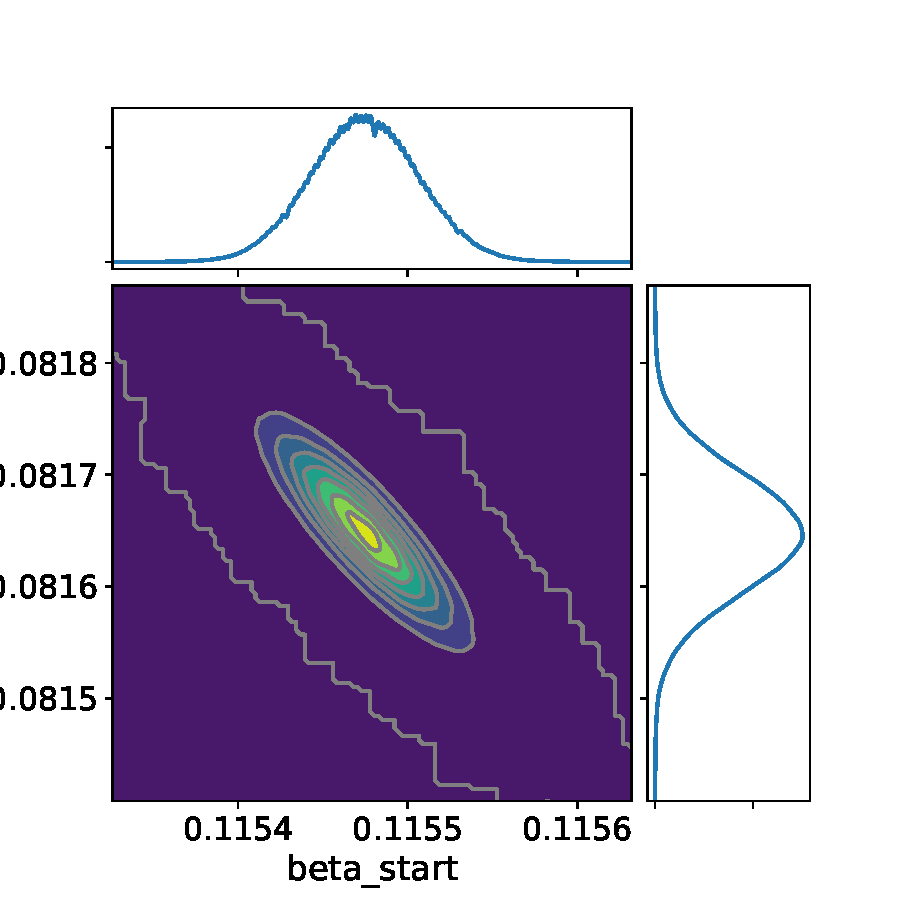
\includegraphics[scale=0.75]{model_joint_betas}
        \caption{Plot of the joint density of $\beta_{start},\beta_{end}$ output by the model.}
        \label{model_joint_betas}
    \end{figure}
    \begin{landscape}
    \begin{figure}
        \centering
        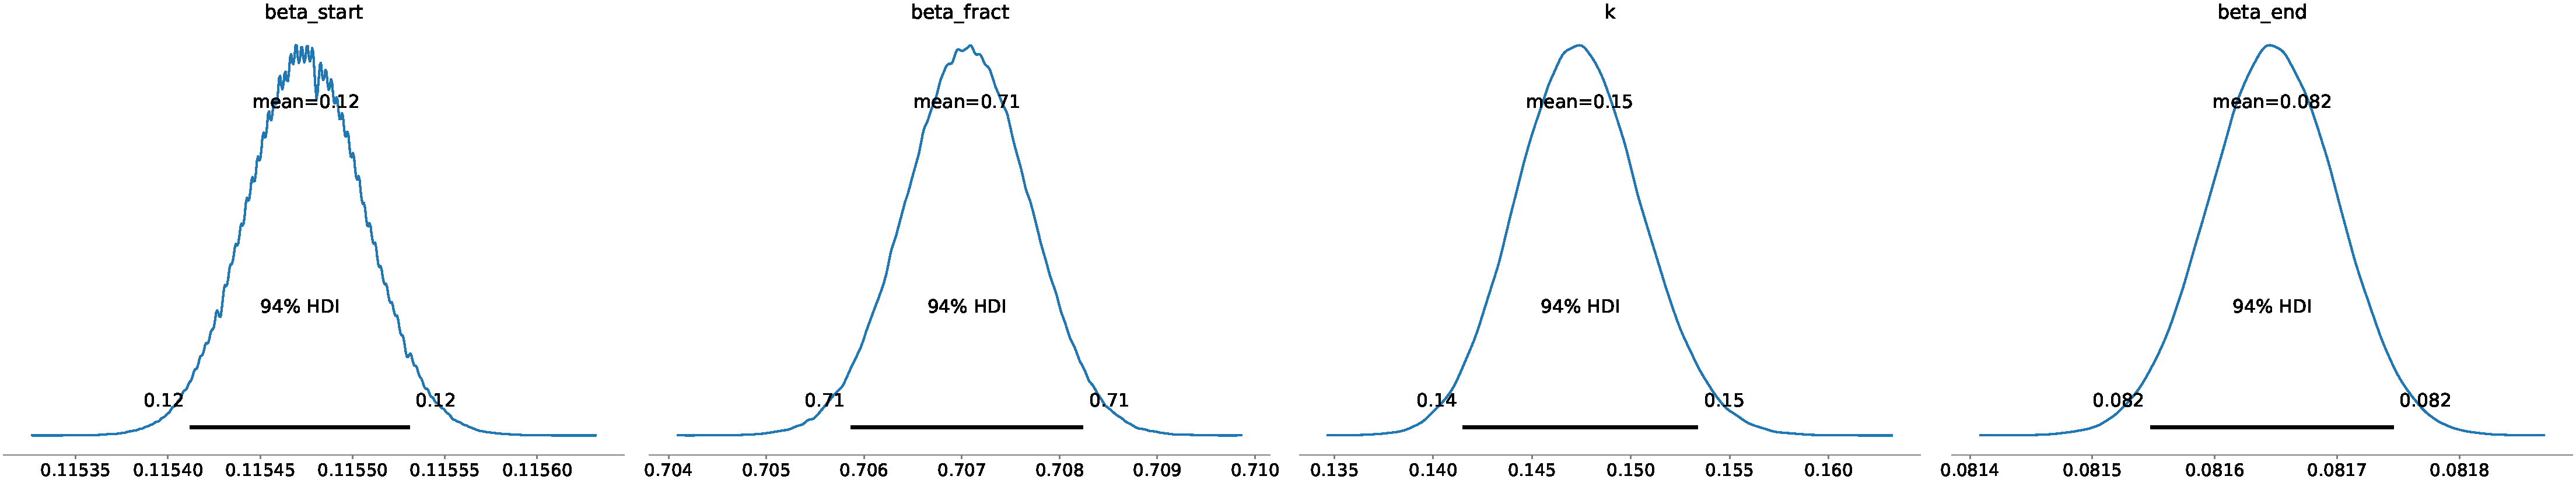
\includegraphics[scale=0.2]{model_posterior}
        \caption{Posterior density plots showing the HDI interval for each estimated parameter.}
        \label{model_posterior}
    \end{figure}
    \begin{figure}
        \centering
        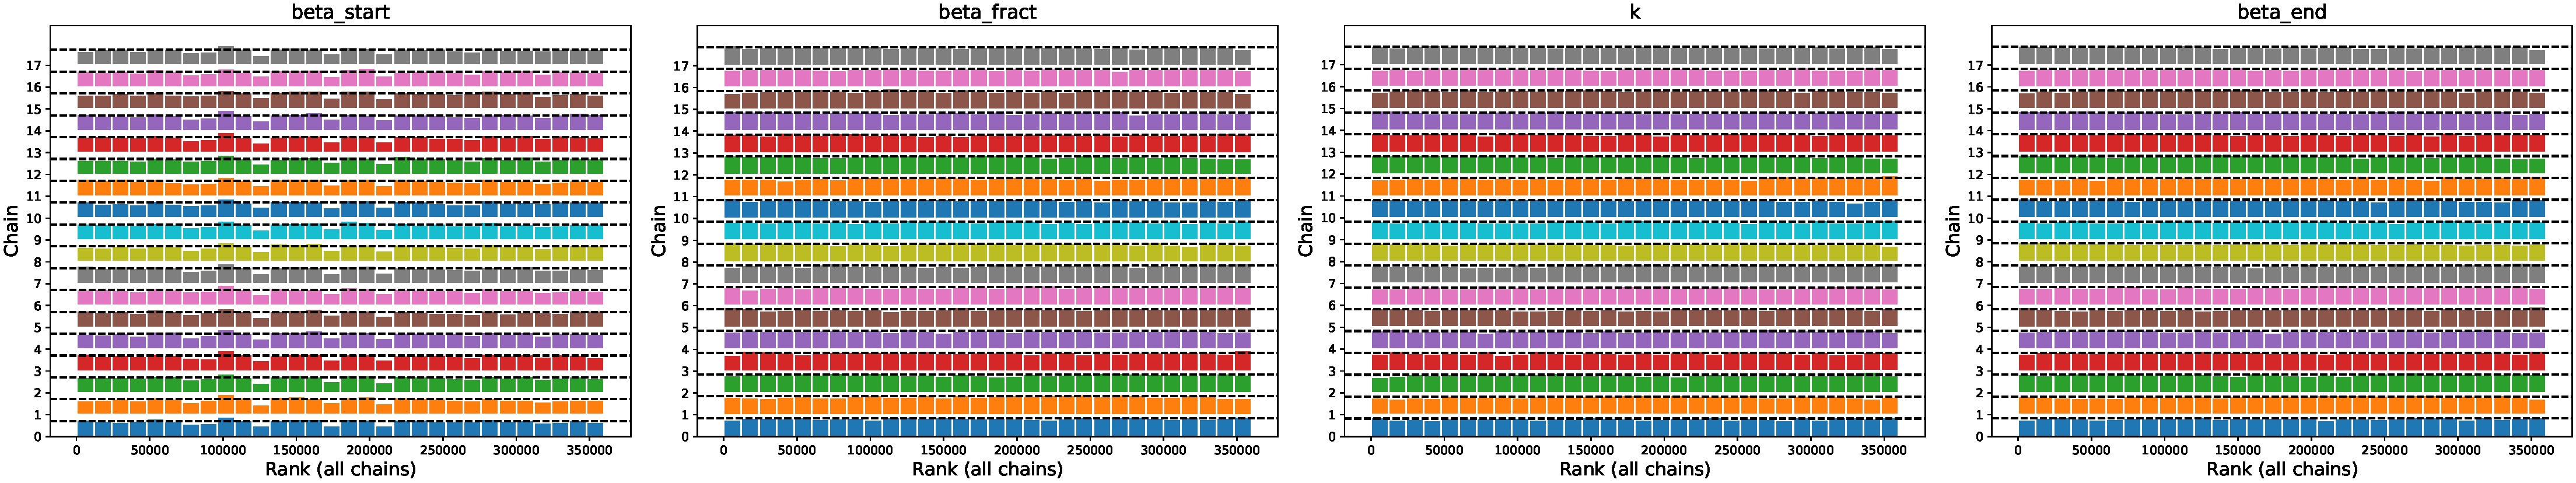
\includegraphics[scale=0.2]{model_rank}
        \caption{Diagnostic plots showing parameter rank for each chain.}
        \label{model_rank}
    \end{figure}
    \begin{figure}
        \centering
        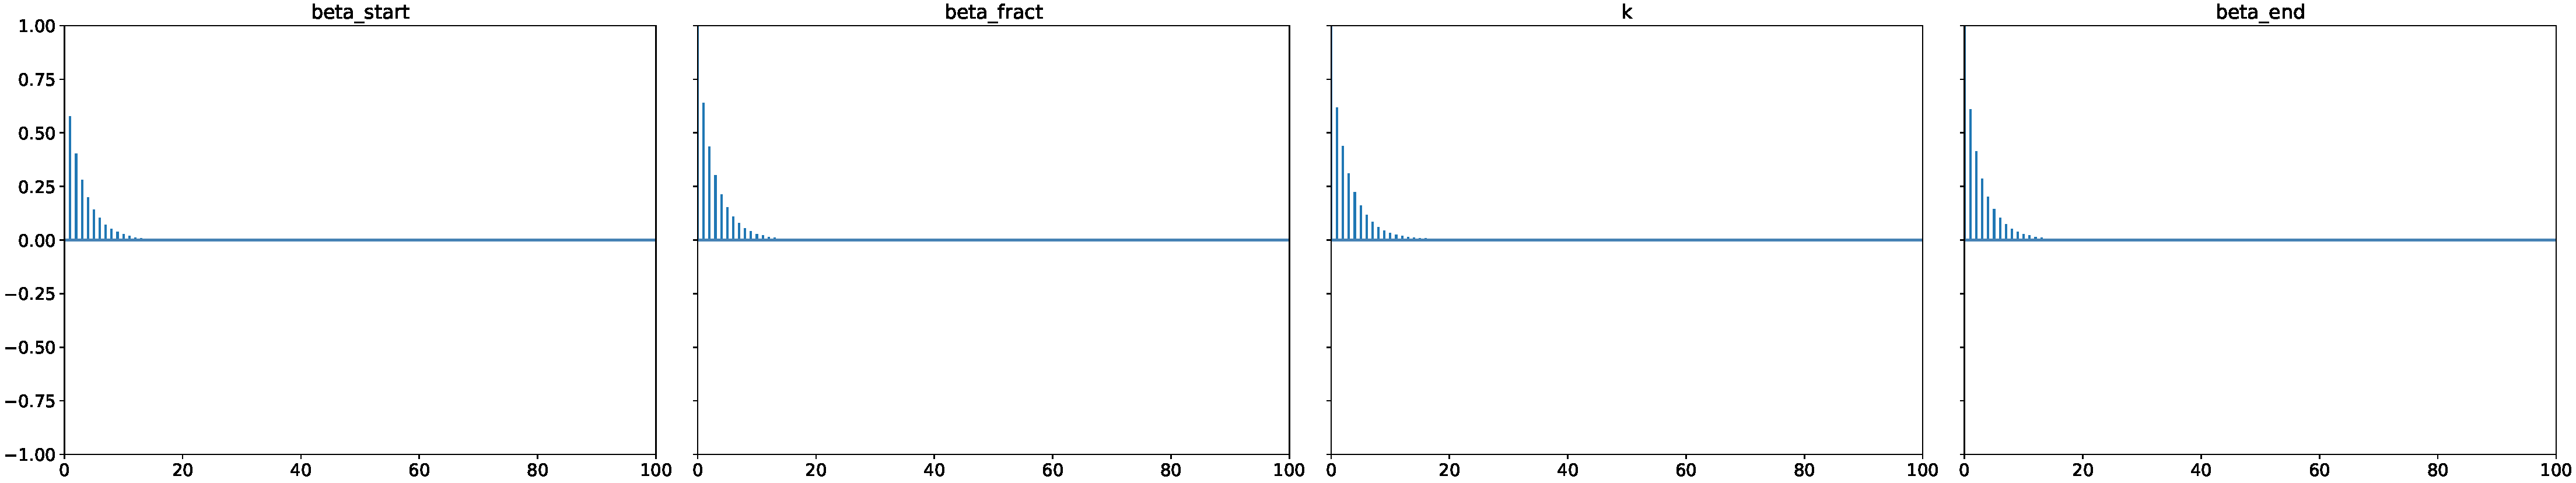
\includegraphics[scale=0.2]{model_autocorrelation}
        \caption{Diagnostic plot showing autocorrelation across all chains.}
        \label{model_autocorrelation}
    \end{figure}
    \end{landscape}

\bibliographystyle{unsrt}
\bibliography{main}

\end{document}
